\documentclass[11pt, a4paper]{article}

% --- 必备宏包 ---
\usepackage[UTF8]{ctex}
\usepackage{amsmath, amsfonts, amssymb}
\usepackage{geometry}
\usepackage{enumerate}
\usepackage{tcolorbox}
\usepackage{caption}
\usepackage{graphicx}
\usepackage{tikz} % 用于重绘第三题的插图
% --- 修复报错的关键行：调用阴影库 ---
\usetikzlibrary{patterns}
\geometry{left=2cm, right=2cm, top=2.5cm, bottom=2.5cm}

\begin{document}

\begin{center}
    \LARGE \bfseries 北京邮电大学 2023—2024 学年第一学期 \\
    《计算电磁学中的数值方法》期末考试试题（A 卷）
\end{center}

\vspace{1em}

% --- 第一题 ---
\section*{一、简答题（10 分）}
试述在计算电磁学的计算方法中，积分方程法和微分方程法各有什么特点？

\begin{tcolorbox}[colback=white, colframe=black, title=【解答】（第一章56页）]
\textbf{1. 积分方程法}
\begin{itemize}
    \item 当关心的物理量是一些“作用量”，例如电压、电流、电荷、电感、电容和电磁能，通常要涉及电磁场强度的积分就要采用积分方程法。
    \item 电磁场的积分方法都需要求解格林函数 (Green's Function)，格林函数解与问题的类型密切相关。
    \item 采用积分方程方法时，处理干扰源和边界条件总是成为分析和建模的关键步骤。
\end{itemize}

\textbf{2. 微分方程法}
\begin{itemize}
    \item 当问题归结为电磁场强度时，就可以由麦氏方程出发得到相应的差分方程，理论分析过程通常比积分方法概念简单，但数值处理的实现要比积分方程难得多。
    \item 微分算子是局域算子，而积分算子是全局性算子。
    \item 最容易发生的问题是企图用数值方法代替理论分析结果。
\end{itemize}
\end{tcolorbox}

% --- 第二题 ---
\section*{二、证明题（10 分）}
试证明：对于任意的非负 $X$ 值，利用蒙特卡洛方法计算的真值与估计值的偏差为：$\left| \widehat{\mathbb{G}}_n - G \right| < \dfrac{X\sigma}{\sqrt{N}}$。

\begin{tcolorbox}[colback=white, colframe=black, title=【解答】（第二章25页）]
根据中心极限定理，只要所确定的无偏估计量是有限的不等于零的方差，则对于任意的非负 $X$ 值均有：
\begin{equation}
    \lim_{N \to \infty} P\left( \frac{\sqrt{N}}{\sigma} \left| \widehat{\mathbb{G}}_n - G \right| < X \right) = \frac{1}{\sqrt{2\pi}} \int_{-X}^{X} e^{-\frac{t^2}{2}} dt
\end{equation}
当 $N$ 足够大时：
\begin{equation}
    \lim_{N \to \infty} P\left( \left| \widehat{\mathbb{G}}_n - G \right| < \frac{X\sigma}{\sqrt{N}} \right) \approx \frac{1}{\sqrt{2\pi}} \int_{-X}^{X} e^{-\frac{t^2}{2}} dt = 1 - \alpha
\end{equation}
其中：
\begin{itemize}
    \item $1 - \alpha$ 为置信水平，$\alpha$ 为置信度。$\sigma$ 为 MC 估计值的标准误差。
    \item $\left| \widehat{\mathbb{G}}_n - G \right| < \dfrac{X\sigma}{\sqrt{N}}$ 的概率由问题的要求确定置信水平。
    \item 由$1 - \alpha$就可按正态分布确定X, 真值与估值的偏差为$\left| \widehat{\mathbb{G}}_n - G \right| < \dfrac{X\sigma}{\sqrt{N}}$
    \item 通常取 $X$ 为 0.6745、1.96、3 分别对应置信水平为 0.5、0.95、0.997。
\end{itemize}
\end{tcolorbox}

% --- 第三题 ---
\section*{三、计算题（10 分）}
设 $I = \int_a^b g(x) dx$，其中 $g(x)$ 满足：1) $g(x) \geq 0$, 2) $\int_{-\infty}^{\infty} g(x) dx = 1$。如何利用 MC 法求解上述积分？给出求解步骤。

\begin{tcolorbox}[colback=white, colframe=black, title=【解答】（第三章8页）]
\begin{minipage}{0.6\textwidth}
根据前辈提供的解题思路，本题可采用 \textbf{投点法 (Hit-or-Miss Method)} 求解：
\begin{enumerate}
    \item \textbf{确定边界}：在区间 $[a, b]$ 上，设 $g(x)$ 的最大值为 $M$。则待求面积包含在矩形 $D = \{ (x, y) \mid a \leq x \leq b, 0 \leq y \leq M \}$ 内。
    \item \textbf{产生随机点}：在矩形 $D$ 内均匀投点。产生两组独立随机数序列 $\xi_i \in [a, b]$ 和 $\eta_i \in [0, M]$，组成随机点 $(\xi_i, \eta_i)$。
    \item \textbf{逻辑判定}：统计随机点落入曲线 $y=g(x)$ 下方区域 $G$ 的次数 $N_{hit}$。判别准则为：
    \begin{equation*}
        \eta_i \leq g(\xi_i)
    \end{equation*}
    \item \textbf{计算积分值}：设总投点数为 $N$，根据面积占比关系，积分值的估计值为：
    \begin{equation*}
        \widehat{I} = \frac{N_{hit}}{N} \times \text{矩形面积} = \frac{N_{hit}}{N} \times M(b-a)
    \end{equation*}
\end{enumerate}
\end{minipage}
\hfill
\begin{minipage}{0.35\textwidth}
\centering
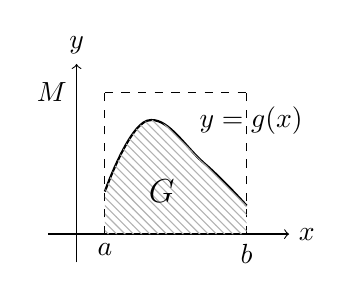
\begin{tikzpicture}[scale=1.8]
    % 坐标轴
    \draw[->] (-0.2,0) -- (1.5,0) node[right] {$x$};
    \draw[->] (0,-0.2) -- (0,1.2) node[above] {$y$};
    % 矩形区域
    \draw[dashed] (0.2,1) -- (1.2,1);
    \draw[dashed] (0.2,0) -- (0.2,1);
    \draw[dashed] (1.2,0) -- (1.2,1);
    % 函数曲线 (示意)
    \draw[thick] plot [smooth, tension=0.7] coordinates {(0.2,0.3) (0.5,0.8) (0.9,0.5) (1.2,0.2)};
    \node[right] at (0.8,0.8) {$y=g(x)$};
    % 填充阴影
    \fill[pattern=north west lines, pattern color=gray!60] (0.2,0) -- plot [smooth, tension=0.7] coordinates {(0.2,0.3) (0.5,0.8) (0.9,0.5) (1.2,0.2)} -- (1.2,0) -- cycle;
    \node at (0.6, 0.3) {\large $G$};
    % 坐标标注
    \node[below] at (0.2,0) {$a$};
    \node[below] at (1.2,0) {$b$};
    \node[left] at (0,1) {$M$};
\end{tikzpicture}
\end{minipage}
\end{tcolorbox}

% --- 第四题 ---
\section*{四、抽样算法题（10 分）}
已知泊松分布的形式为：$P(X=n) = P_n = e^{-\lambda} \dfrac{\lambda^n}{n!}$，如何利用抽样算法得到服从泊松分布的子样或者随机变量？

\begin{tcolorbox}[colback=white, colframe=black, title=【解答】（第二章87页）]
对于 Poisson 分布，在 $t=1$ 情况下：
\begin{equation}
    P(X=n) = P_n = e^{-\lambda} \frac{\lambda^n}{n!}
\end{equation}
设 $\xi$ 为 $[0, 1]$ 上的均匀分布随机数。若下式成立：
\begin{equation}
    \sum_{i=0}^{n-1} \frac{\lambda^i}{i!} < e^{\lambda} \xi \leq \sum_{i=0}^{n} \frac{\lambda^i}{i!}
\end{equation}
则随机变量取值 $\xi_F = n$。
\end{tcolorbox}

% --- 第五题 ---
\section*{五、数值方法题（10 分）}
已知三阶龙格-库塔格式为：
\begin{equation}
\begin{cases}
    y_{n+1} = y_n + \dfrac{1}{6}(K_1 + 4K_2 + K_3) \\
    K_1 = h f(x_n, y_n) \\
    K_2 = h f(x_n + h/2, y_n + K_1/2) \\
    K_3 = h f(x_n + h, y_n - K_1 + 2K_2) \\
    y(x_{n+1}) - y_{n+1} = O(h^4) \text{}
\end{cases}
\end{equation}
对于方程 $\dfrac{dy}{dx} = y - \dfrac{2x}{y}, y|_{x=0}=1$，取步长 $h=0.1$ 进行近似计算。

\begin{tcolorbox}[colback=white, colframe=black, title=【解答】（第四章）]
已知 $f(x, y) = y - \dfrac{2x}{y}, x_0=0, y_0=1, h=0.1$。\\
虽然 PPT 示例为四阶计算，本题严格按照试卷要求的\textbf{三阶格式}计算第一步：
\begin{enumerate}
    \item $K_1 = 0.1 \times f(0, 1) = 0.1000$
    \item $K_2 = 0.1 \times f(0.05, 1.05) = 0.1 \times (1.05 - \frac{0.1}{1.05}) \approx 0.0955$
    \item $K_3 = 0.1 \times f(0.1, 1 - 0.1 + 2 \times 0.0955) \approx 0.0908$
    \item $y_1 = 1 + \dfrac{1}{6}(0.1 + 4 \times 0.0955 + 0.0908) \approx 1.0955$
\end{enumerate}
精确解为 $y(0.1) = \sqrt{1 + 2(0.1)} \approx 1.0954$。
\end{tcolorbox}

% --- 第六题 ---
\section*{六、(10 分)}
对于题六图所示的外法线与网格线不重合情况，边界结点上的外向法线方向与水平夹角为 $\alpha$。如何分析第三类边界 $\left.\left[\varphi+f_{1}\left(\overrightarrow{r^{\prime}}, t\right) \frac{\partial \varphi}{\partial n}\right]\right|_{S}=f_{2}\left(\overrightarrow{r^{\prime}}, t\right)$ 的差分格式？

\begin{tcolorbox}[colback=white, colframe=black, title=【解答】（第四章）]
\begin{minipage}{0.55\textwidth}
当外法线与网格线不重合时，边界结点上的法向导数是在 $x$ 和 $y$ 方向导数在法向的投影组合，即采用 \textbf{投影法} 进行离散化：
\begin{enumerate}
    \item \textbf{法向导数分解}：
    在结点 0 处，法向导数可以表示为：
    \begin{equation*}
        \left( \frac{\partial \varphi}{\partial n} \right)_0 = \left[ \frac{\partial \varphi}{\partial x} \cos \alpha + \frac{\partial \varphi}{\partial y} \sin \alpha \right]_0
    \end{equation*}
    \item \textbf{差分离散化}：
    利用相邻网格结点 3 和 2 进行一阶差分近似：
    \begin{equation*}
        \left( \frac{\partial \varphi}{\partial n} \right)_0 \approx \frac{\varphi_0 - \varphi_3}{h} \cos \alpha + \frac{\varphi_0 - \varphi_2}{h} \sin \alpha
    \end{equation*}
    \item \textbf{最终差分格式}：
    代入第三类边界条件方程得：
    \begin{equation*}
        \varphi_0 + f_1(r_0) \left( \frac{\varphi_0 - \varphi_3}{h} \cos \alpha + \frac{\varphi_0 - \varphi_2}{h} \sin \alpha \right) = f_2(r_0)
    \end{equation*}
\end{enumerate}
\end{minipage}
\hfill
\begin{minipage}{0.4\textwidth}
\centering
% 在这里插入你从 PPT 截取的图片文件
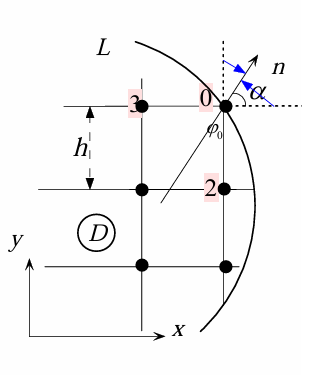
\includegraphics[width=\textwidth]{6.png} 
\captionof{figure}{投影法分析图示}
\end{minipage}
\end{tcolorbox}

% --- 第七题 ---
\section*{七、(10 分)}
试推导如下方程的时域有限差分格式：
\begin{equation*}
    \frac{\partial E_x}{\partial t} = \frac{1}{\epsilon} \left( \frac{\partial H_z}{\partial y} - \frac{\partial H_y}{\partial z} \right)
\end{equation*}

\begin{tcolorbox}[colback=white, colframe=black, title=【解答】（第五章-1 27页）]
\begin{minipage}{0.55\textwidth}
\textbf{1. 离散化推导（以 $E_x$ 为例）}：
\begin{itemize}
    \item \textbf{取样定义}：在 Yee 元胞中，$E_x$ 分量在 $(i+1/2, j, k)$ 点取样，时间步位于整数时刻 $n$。
    \item \textbf{中心差分}：对时间导数在 $n+1/2$ 时刻应用中心差分，空间导数在对应的半步长处应用中心差分。
    \item \textbf{迭代格式}：整理得到 $E_x$ 的显式更新方程：
\end{itemize}
\begin{align*}
    E_x^{n+1}(i+\frac{1}{2}, j, k) = & E_x^n(i+\frac{1}{2}, j, k) + \frac{\Delta t}{\epsilon} \bigg[ \\
    & \frac{H_z^{n+\frac{1}{2}}(i+\frac{1}{2}, j+\frac{1}{2}, k) - H_z^{n+\frac{1}{2}}(i+\frac{1}{2}, j-\frac{1}{2}, k)}{\Delta y} \\
    & - \frac{H_y^{n+\frac{1}{2}}(i+\frac{1}{2}, j, k+\frac{1}{2}) - H_y^{n+\frac{1}{2}}(i+\frac{1}{2}, j, k-\frac{1}{2})}{\Delta z} \bigg]
\end{align*}
\end{minipage}
\hfill
\begin{minipage}{0.4\textwidth}
\centering
% 请在此替换为你从 PPT 截图的 Ex 采样示意图
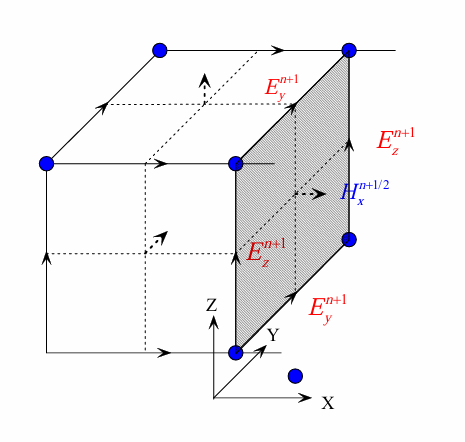
\includegraphics[width=\textwidth]{7.png}
\captionof{figure}{Yee 元胞采样点分布}
\end{minipage}

\vspace{1em}
\hrule
\vspace{1em}

\textbf{2. 其他场分量的 FDTD 差分格式汇总}：
\begin{itemize}
    \item \textbf{磁场分量 ($H$ 场) 的更新格式}：
    \begin{align*}
        H_x^{n+\frac{1}{2}} = H_x^{n-\frac{1}{2}} & + \frac{\Delta t}{\mu} \left[ \frac{E_y^n(k+1) - E_y^n(k)}{\Delta z} - \frac{E_z^n(j+1) - E_z^n(j)}{\Delta y} \right] \\
        H_y^{n+\frac{1}{2}} = H_y^{n-\frac{1}{2}} & + \frac{\Delta t}{\mu} \left[ \frac{E_z^n(i+1) - E_z^n(i)}{\Delta x} - \frac{E_x^n(k+1) - E_x^n(k)}{\Delta z} \right] \\
        H_z^{n+\frac{1}{2}} = H_z^{n-\frac{1}{2}} & + \frac{\Delta t}{\mu} \left[ \frac{E_x^n(j+1) - E_x^n(j)}{\Delta y} - \frac{E_y^n(i+1) - E_y^n(i)}{\Delta x} \right]
    \end{align*}
    
    \item \textbf{电场分量 ($E$ 场) 的更新格式}：
    \begin{align*}
        E_y^{n+1} = E_y^n & + \frac{\Delta t}{\epsilon} \left[ \frac{H_x^{n+\frac{1}{2}}(k+\frac{1}{2}) - H_x^{n+\frac{1}{2}}(k-\frac{1}{2})}{\Delta z} - \frac{H_z^{n+\frac{1}{2}}(i+\frac{1}{2}) - H_z^{n+\frac{1}{2}}(i-\frac{1}{2})}{\Delta x} \right] \\
        E_z^{n+1} = E_z^n & + \frac{\Delta t}{\epsilon} \left[ \frac{H_y^{n+\frac{1}{2}}(i+\frac{1}{2}) - H_y^{n+\frac{1}{2}}(i-\frac{1}{2})}{\Delta x} - \frac{H_x^{n+\frac{1}{2}}(j+\frac{1}{2}) - H_x^{n+\frac{1}{2}}(j-\frac{1}{2})}{\Delta y} \right]
    \end{align*}
\end{itemize}
\end{tcolorbox}

% --- 第八题 ---
\section*{八、(10 分)}
试推导并分析在时域有限差分法中，对于 Yee 网格抽样标准网格的大小选取为 $\Delta s = \lambda / 10$ 的依据。

\begin{tcolorbox}[colback=white, colframe=black, title=【解答】（第五章-1 61页）]
\begin{minipage}{0.55\textwidth}
在时域有限差分法（FDTD）中，空间步长 $\Delta s$ 的选取直接影响数值色散和计算精度。其选取依据分析如下：
\begin{enumerate}
    \item \textbf{网格尺寸对比分析}：
    \begin{itemize}
        \item 当 $\Delta s = \lambda/5$ 时，网格尺寸比要求的标准网格大，色散误差显著。
        \item 当 $\Delta s = \lambda/10$ 时，基本满足标准网格要求，能较好地抑制数值色散。
        \item 当 $\Delta s = \lambda/20$ 时，网格比要求更细，精度更高但计算资源消耗剧增。
    \end{itemize}

    \item \textbf{数值色散与相速度}：
    相速度随空间步长的增加而减小，直到减小为零。不同的入射角下，相速度下降对应的 $\Delta s$ 极限不同；在 45 度入射角处，急剧下降的临界步长值最大。

    \item \textbf{传播极限与低通滤波特性}：
    \begin{itemize}
        \item Yee 网格存在空间步长极限。超过该极限，电磁波将不能在空间中传播。
        \item 给定的 Yee 网格相当于一个低通滤波器，会导致高频分量被截断，给宽频脉冲计算带来困难。
    \end{itemize}

    \item \textbf{结论}：
    为了保证波形在传播过程中不失真并兼顾计算效率，通常取 $\Delta s = \lambda / 10$ 作为标准网格步长。
\end{enumerate}
\end{minipage}
\hfill
\begin{minipage}{0.4\textwidth}
\centering
% 请在此替换为你从 PPT 截图的数值色散关系图 (vp/c 与 Δs 的关系)
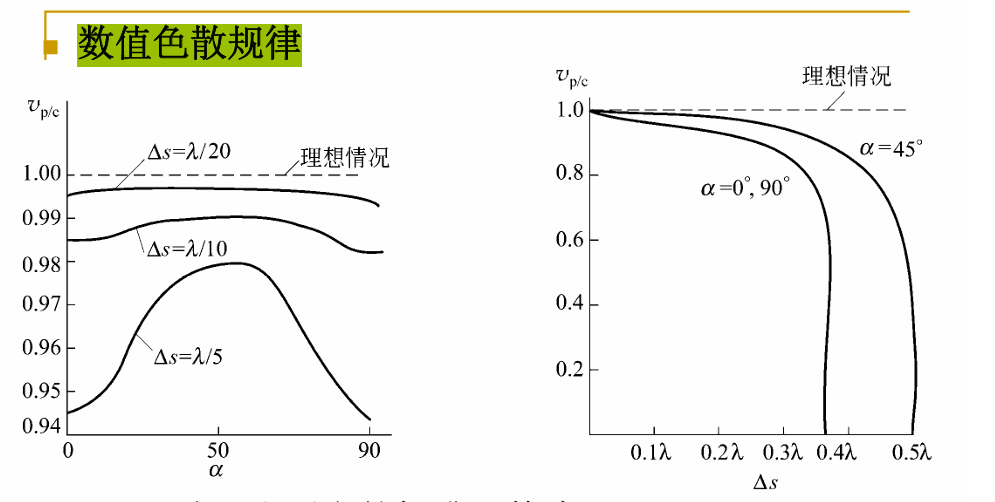
\includegraphics[width=\textwidth]{8.png}
\captionof{figure}{数值色散与步长关系图}
\end{minipage}
\end{tcolorbox}

% --- 第九题 ---
\section*{九、(10 分)}
为什么在求解散射场时，往往采用近场-远场变换的方法？试在直接坐标系下说明近场-远场变换原理。

\begin{tcolorbox}[colback=white, colframe=black, title=【解答】（第五章-3）]
\begin{enumerate}
    \item \textbf{采用近场-远场变换的原因}：
    \begin{itemize}
        \item \textbf{区域划分}：在数值计算中，网格空间被划分为总场区和散射场区，散射体位于总场区中，而散射的全部信息由散射场区获取。
        \item \textbf{存储限制}：由于计算机存储空间的限制，散射场区不可能选得很大，导致网格空间内的散射场区实际上属于散射近场。
        \item \textbf{目标需求}：通常雷达散射截面 (RCS) 等目标散射特征定义在远区场，为了由有限区域内的近场特征求得远场特征，必须寻求近/远场变换方法。
    \end{itemize}

    \item \textbf{近场-远场变换原理}：
    \begin{itemize}
        \item \textbf{构建包面}：在完全包围散射体的位置设置一个具有简单形状的虚设表面 $S_a$（如由长方体的六个平面组成的包面）。
        \item \textbf{提取近场数据}：在计算过程中，解出该虚设表面 $S_a$ 上散射近场的电场及磁场的切向分量。
        \item \textbf{等效源转化}：应用等效原理，将 $S_a$ 面上的切向场分量转化为等效电流和等效磁流，将其作为辐射源。
        \item \textbf{积分求解}：利用熟知的矢量位 (Vector Potential) 公式，通过对等效源进行空间积分，求解出远区散射场。
    \end{itemize}
    \item \textbf{算法优势}：虚设表面 $S_a$ 的设置不依赖于实际散射体的形状，使得算法具有极强的通用性。
\end{enumerate}
\end{tcolorbox}

% --- 第十题 ---
\section*{十、(10 分)}
试用点匹配法给出如下方程的二阶矩量法近似求解：
\begin{equation*}
    \frac{d^2 f}{dx^2} = 1 + 4x^2, \quad 0 < x < 1
\end{equation*}
假设边界条件为 $f(0) = f(1) = 0$。

\begin{tcolorbox}[colback=white, colframe=black, title=【解答】（第八章-Gemini作答）]
\textbf{1. 选取基函数}
根据矩量法原理，选取满足边界条件 $f(0)=0$ 和 $f(1)=0$ 的全域基函数。对于二阶近似，取 $N=2$，令近似解为：
\begin{equation*}
    \hat{f}(x) = a_1 \phi_1(x) + a_2 \phi_2(x) = a_1(x - x^2) + a_2(x^2 - x^3)
\end{equation*}

\textbf{2. 建立余数方程}
定义算子 $L = \dfrac{d^2}{dx^2}$，源项 $g(x) = 1 + 4x^2$。余数方程为：
\begin{align*}
    R(x) &= L\hat{f}(x) - g(x) = \frac{d^2}{dx^2} [a_1(x - x^2) + a_2(x^2 - x^3)] - (1 + 4x^2) \\
    &= -2a_1 + a_2(2 - 6x) - (1 + 4x^2)
\end{align*}

\textbf{3. 点匹配法求解}
选取计算区域 $[0, 1]$ 内的两个匹配点 $x_1 = 1/3$ 和 $x_2 = 2/3$，令 $R(x_i) = 0$：
\begin{itemize}
    \item 当 $x = 1/3$ 时：
    \begin{equation*}
        -2a_1 + a_2(2 - 2) - (1 + \frac{4}{9}) = 0 \implies -2a_1 = \frac{13}{9} \implies a_1 = -\frac{13}{18}
    \end{equation*}
    \item 当 $x = 2/3$ 时：
    \begin{equation*}
        -2a_1 + a_2(2 - 4) - (1 + \frac{16}{9}) = 0 \implies -2a_1 - 2a_2 = \frac{25}{9}
    \end{equation*}
\end{itemize}
联立求解得到系数：
\begin{equation*}
    a_1 = -\frac{13}{18}, \quad a_2 = -\frac{12}{18} = -\frac{2}{3}
\end{equation*}

\textbf{4. 最终近似解}
将系数回代得到近似解表达式：
\begin{equation*}
    \hat{f}(x) = -\frac{13}{18}x + \frac{1}{18}x^2 + \frac{2}{3}x^3
\end{equation*}
\end{tcolorbox}

\end{document}
